\section{\acs{LSTM}}
\begin{table}[h]
\centering
\begin{tabular}{|c|c|c|c|c|c|c|c||c|}
\hline
\diaghead{\theadfont xxxxxxxxxxxxxxxxxxxx}%
{\textbf{LSTM-Blöcke}}{\textbf{Iterationen}}& \textbf{100} & \textbf{200} & \textbf{300} & \textbf{400} & \textbf{700} & \textbf{1000} \\
 \hline
8&50,16\%&43,33\%&30,80\%&27,13\%&23,31\%&22,59\%\\ \hline
10&51,39\%&40,61\%&35,54\%&29,96\%&24,65\%&21,13\%\\ \hline
12&46,52\%&39,99\%&34,65\%&33,01\%&28,59\%&25,37\%\\ \hline
14&54,61\%&43,09\%&39,90\%&34,71\%&27,90\%&23,72\%\\ \hline
16&39,24\%&31,48\%&26,89\%&24,44\%&17,58\%&13,97\%\\ \hline
18&45,33\%&34,71\%&28,44\%&25,63\%&18,35\%&15,70\%\\ \hline
20&48,40\%&37,18\%&31,42\%&30,02\%&22,80\%&18,38\%\\ \hline
\end{tabular} 
\caption[Tests für LSTM-Block Anzahl]{Tests um Anzahl der LSTM-Blöcke herauszufinden. Werte geben Fehlerrate des Netzwerks an. Das Trainigsverfahren ist \texttt{RProp}. Outputlayerart ist \texttt{Softmax}. }
\label{tab:neurontests}
\end{table}

\begin{table}[h]
\centering
\begin{tabular}{|c|c|c|c|c|c|c|}
\hline
\diaghead{\theadfont xxxxxxxxxxxxxxxxxxxx}%
{\textbf{Layerart}}{\textbf{Iterationen}}& \textbf{500} & \textbf{1000} & \textbf{1500}\\
 \hline
linear&30,42\%&22,22\%&19,57\%\\\hline
sigmoid&23,74\%&19,62\%&17,25\%\\\hline
softmax&23,57\%&18,70\%&16,25\%\\\hline
\end{tabular} 
\caption[Tests für Outputlayer]{Tests um Art des Outputlayer zu bestimmen. Werte geben Fehlerrate des Netzwerks an. Das Trainigsverfahren ist \texttt{RProp}. Die Anzahl der LSTM-Blöcke ist 16. }
\label{tab:outlayertests}
\end{table}

 
\begin{table}
\centering
\begin{tabular}{|l|c|c|c|c|c|c|}
\hline
\diaghead{\theadfont xxxxxxxxxxxxxxxxxxxx}%
{\textbf{LSTM-Blöcke}}{\textbf{Iterationen}}& \textbf{250} & \textbf{500}\\
 \hline
8&55,40\%&84,02\%\\\hline
10&64,05\%&70,09\%\\\hline
12&65,97\%&57,35\%\\\hline
14&64,41\%&45,40\%\\\hline
16&64,62\%&67,35\%\\\hline
18&70,48\%&67,50\%\\\hline
\end{tabular} 
\caption[Tests für Trainigverfahren]{Tests um Ergebnisverhalten des Trainingverfahrens Backpropagation zu zeigen. Werte geben Fehlerrate des Netzwerks an. Outputlayerart ist \texttt{Softmax}. Momentunmparameter ist 0,01. }
\label{tab:outlayertests}
\end{table}

\begin{sidewaystable}[h]
\centering
\begin{tabular}{|c|c|c|c|c|c|c|c|c|c|c|}
\hline
 \textbf{Fold} & \textbf{Cut} & \textbf{Peephole} & \diaghead{\theadfont xxxxxxxxxxxxxxxxxxxx}%
{\textbf{LSTM-Blöcke}}{\textbf{Iterationen}} & \textbf{250} & \textbf{500} & \textbf{750} & \textbf{1000} & \textbf{1250} & \textbf{1500} & \textbf{Zeit} (Mittel)\\
&&&&&&&&&& min/Iteration\\
 \hline 
 \multirow{12}{*}{1}&\multirow{4}{*}{0}&\multirow{2}{*}{true}&16&28,39\%&27,30\%&26,54\%&27,19\%&26,33\%&26,33\%&\multirow{12}{*}{1,56}\\\cline{4-10}
  & & &18&29,14\%&28,06\%&26,00\%&26,89\%&25,14\%&26,11\%&\\\cline{3-10}
  & &\multirow{2}{*}{false}&16&30,55\%&29,58\%&26,44\%&26,76\%&27,09\%&26,11\%&\\\cline{4-10}
  & & &18&26,65\%&26,22\%&25,35\%&24,81\%&25,35\%&25,89\%&\\\cline{2-10}
  
  &\multirow{4}{*}{16}&\multirow{2}{*}{true}&16&36,73\%&35,21\%&33,37\%&32,61\%&32,72\%&32,29\%&\\\cline{4-10}
  & & &18&33,69\%&31,20\%&29,90\%&29,47\%&29,25\%&29,04\%&\\\cline{3-10}
  & &\multirow{2}{*}{false}&16&30,44\%&30,44\%&29,36\%&29,79\%&28,93\%&29,79\%&\\\cline{4-10}
  & & &18&30,34\%&27,95\%&27,95\%&28,17\%&27,74\%&28,17\%&\\\cline{2-10}
  
  &\multirow{4}{*}{24}&\multirow{2}{*}{true}&16&33,59\%&32,07\%&31,53\%&32,07\%&29,47\%&30,34\%&\\\cline{4-10}
  & & &18&35,75\%&33,69\%&29,04\%&27,74\%&31,09\%&30,77\%&\\\cline{3-10}
  & &\multirow{2}{*}{false}&16&33,15\%&33,15\%&32,39\%&32,18\%&31,96\%&31,42\%&\\\cline{4-10}
  & & &18&32,50\%&31,20\%&30,01\%&29,79\%&29,47\%&28,71\%&\\\hline
  
  \multirow{12}{*}{2}&\multirow{4}{*}{0}&\multirow{2}{*}{true}&16&35,54\%&31,96\%&31,74\%&31,64\%&29,14\%&29,14\%&\multirow{12}{*}{0,81}\\\cline{4-10}
  & & &18&33,59\%&31,64\%&29,36\%&29,58\%&27,74\%&27,52\%&\\\cline{3-10}
  & &\multirow{2}{*}{false}&16&34,99\%&32,07\%&30,34\%&29,58\%&28,93\%&26,11\%&\\\cline{4-10}
  & & &18&36,94\%&33,91\%&31,96\%&32,18\%&26,44\%&28,93\%&\\\cline{2-10}

  &\multirow{4}{*}{16}&\multirow{2}{*}{true}&16&33,69\%&32,74\%&30,01\%&29,98\%&25,14\%&25,79\%&\\\cline{4-10}
  & & &18&33,26\%&31,74\%&30,01\%&29,69\%&26,44\%&27,63\%&\\\cline{3-10}
  & &\multirow{2}{*}{false}&16&32,50\%&30,66\%&28,49\%&27,63\%&27,74\%&27,30\%&\\\cline{4-10}
  & & &18&35,64\%&35,10\%&31,85\%&31,09\%&31,31\%&30,34\%&\\\cline{2-10}
  
  &\multirow{4}{*}{24}&\multirow{2}{*}{true}&16&35,97\%&34,56\%&34,45\%&33,48\%&33,04\%&31,42\%&\\\cline{4-10}
  & & &18&33,26\%&32,72\%&29,58\%&33,48\%&32,61\%&32,39\%&\\\cline{3-10}
  & &\multirow{2}{*}{false}&16&35,32\%&34,74\%&32,61\%&32,29\%&29,04\%&28,60\%&\\\cline{4-10}
  & & &18&31,85\%&30,99\%&30,34\%&28,71\%&28,91\%&27,95\%&\\
\hline
\end{tabular} 
\caption[Tests für Daten und LSTM-Netz]{Tests um Parameter für Datenvorverarbeitung und LSTM-Netz zu finden. Werte geben Fehlerrate des Netzwerks an. Das Trainigsverfahren ist \texttt{RProp}. Outputlayerart ist \texttt{Softmax}. }
\label{tab:inputtests}
\end{sidewaystable}

\begin{figure}[h]
  \begin{center}
  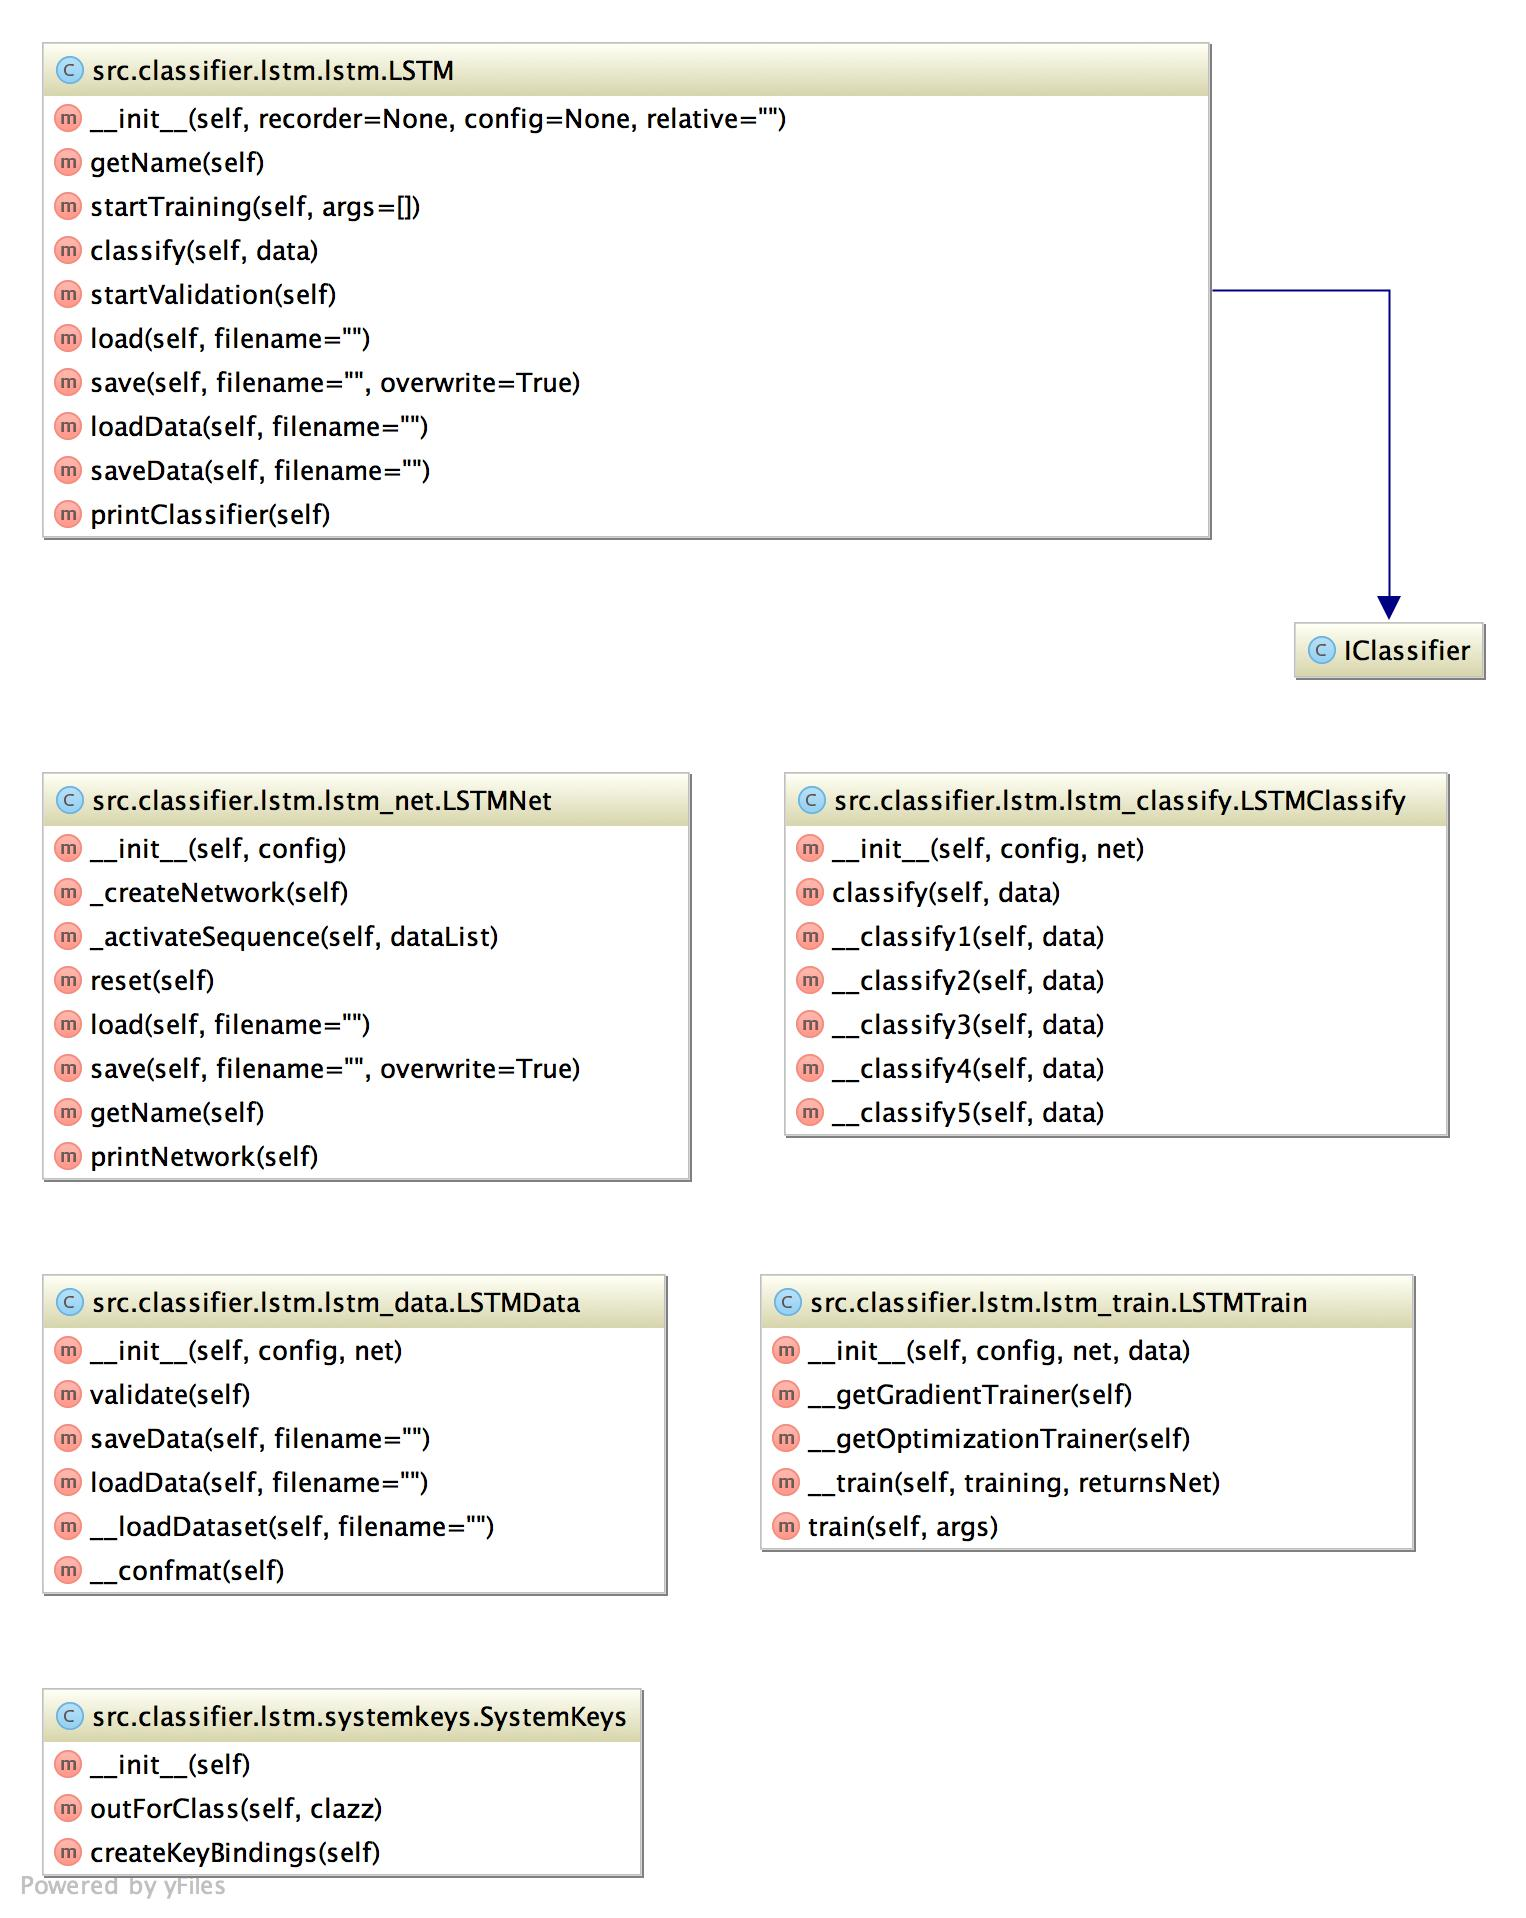
\includegraphics[width=0.95\textwidth]{lstm/diagram}
  \caption[\acs{LSTM} Klassendiagramm]{Klassendiagramm des \acs{LSTM} Moduls innerhalb des Gestenerkennungsprogramm. }
  \label{fig:lstm_class}
  \end{center}
\end{figure}  